
\documentclass[11pt,a4paper,sans]{moderncv} % Font sizes: 10, 11, or 12; paper sizes: a4paper, letterpaper, a5paper, legalpaper, executivepaper or landscape; font families: sans or roman

\moderncvstyle{banking} % CV theme - options include: 'casual' (default), 'classic', 'oldstyle' and 'banking'
\moderncvcolor{blue} % CV color - options include: 'blue' (default), 'orange', 'green', 'red', 'purple', 'grey' and 'black'

\usepackage{lipsum} % Used for inserting dummy 'Lorem ipsum' text into the template
\usepackage[hyperref, UTF8]{ctex}
\usepackage[absolute,overlay]{textpos}
\usepackage[scale=0.85]{geometry} % Reduce document margins
%\setlength{\hintscolumnwidth}{3cm} % Uncomment to change the width of the dates column
%\setlength{\makecvtitlenamewidth}{10cm} % For the 'classic' style, uncomment to adjust the width of the space allocated to your name

%----------------------------------------------------------------------------------------
%	NAME AND CONTACT INFORMATION SECTION
%----------------------------------------------------------------------------------------
%\name{张胜威}{}
\title{ZJU CAD}

%% {%
%% \let\oldmakecvtitle\makecvtitle
%% \renewcommand*{\makecvtitle}{%
%%   \oldmakecvtitle%
%%   {\raggedleft\includegraphics[scale=0.8]{pictures/picture.jpg}\par}%
%% }%
%% }

\firstname{} % Your first name
\familyname{张胜威} % Your last name

% All information in this block is optional, comment out any lines you don't need
%\title{Curriculum Vitae}
\address{浙江省杭州市}{浙大紫金港蒙民伟楼416}
\mobile{(0571) 15700079643}
\email{wegatron@hotmail.com}

\begin{document}

%% \hskip -3.5cm {\makecvtitle}
%% \begin{textblock}{0}(10.5,1)
%%   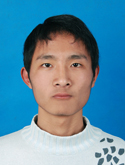
\includegraphics[width=30mm]{zsw}\par
%% \end{textblock}

\makecvtitle % Print the CV title

\section{教育经历}
\cventry{2013.9--2016.4}{硕士}{浙江大学}{浙江省杭州市}{\textit{计算机应用技术CAD\&CG国家重点实验室}}{方向:三维模型处理}
\cventry{2008.9--2012.6}{本科}{浙江工商大学}{浙江省杭州市}{\textit{软件工程}}{}

\section{工作\&实习}
\cventry{2015.6--2015.8}{杭州先临(实习)}{}{}{}{使用多种方案主要包括双边滤波和局部曲面拟合(Moving Least Squares)来去除扫描下来的三维模型中的噪声,使得模型表面更加光滑而又尽可能与原模型保持一致。}

\cventry{2012.6--2012.10}{杭州迪普科技(工作)}{}{}{}{参与了WebShield网站防护系统项目,完善网站备份功能,添加了备份排除目录(文件)列表。并对WebShield系统进行了一系列测试,比如SQL注入,XSS跨站脚本等。参与了WebScanner网站漏洞扫描系统项目,将单线程扫描改为多线程扫描,对扫描过程中所获得的网站目录进行一个hash分配给不同的线程扫描。}

\section{项目经历}
\cventry{2014.10--2015.5}{ShapeMaker}{}{}{}{一个方便普通用户DIY三维模型的软件(cut模型的选择、裁剪,paste模型元素的粘贴, deform形变等)。\newline{}%
 主要工作:基本上所有UI的实现,(包括UI框架qt+open scene graph+finite state machine的重构,显示和操作工具如选取工具,粘贴工具等),以及一些算法的实现如Vector Field形变算法的实现(论文"Vector Field Based Shape Deformations")。}

\cventry{2013.9--2014.9}{Embedded thin shell simulation}{}{}{}{为了更加高效率的模拟弹性体的表面细节,我们在一个粗糙的体网格上嵌一张精细的面网格,以体网格驱动表面网格的形变,从而可以较快速的模拟一个表面具有丰富细节的弹性体模型的运动.\newline{}%
主要工作:code的移植(linux转windows)使用了一个小trick使得无法在windows的库,在需要使用的时候才load而又不影响以前的code。简单的碰撞检测极其处理的实现。Maya插件(让Maya能够调用该算法)。}

\section{技术能力}
\begin{itemize}
\item 熟练使用c++、Linux
\item 熟悉操作系统、计算机网络和程序运行的基本原理,基本的算法和数据结构
\item 英六级:542
\end{itemize}


\clearpage

%% \recipient{HR Department}{Corporation\\123 Pleasant Lane\\12345 City, State} % Letter recipient
%% \date{\today} % Letter date
%% \opening{Dear Sir or Madam,} % Opening greeting
%% \closing{Sincerely yours,} % Closing phrase
%% \enclosure[Attached]{curriculum vit\ae{}} % List of enclosed documents

%% \makelettertitle % Print letter title

%% \lipsum[1-3] % Dummy text

%% \makeletterclosing % Print letter signature

%----------------------------------------------------------------------------------------

\end{document}
